\documentclass{article}

\usepackage{graphicx}
\usepackage{tikz}
\usepackage{tikzsymbols}
\usetikzlibrary{calc,patterns,shapes.geometric}
\pagestyle{empty}
\usepackage[margin=0pt]{geometry}
\geometry{papersize={14in,12in}}

\def\centerarc[#1](#2)(#3:#4:#5){\draw[#1] ($(#2)+({#5*cos(#3)},{#5*sin(#3)})$) arc (#3:#4:#5);}

\begin{document}
	\begin{figure}
		\centering
		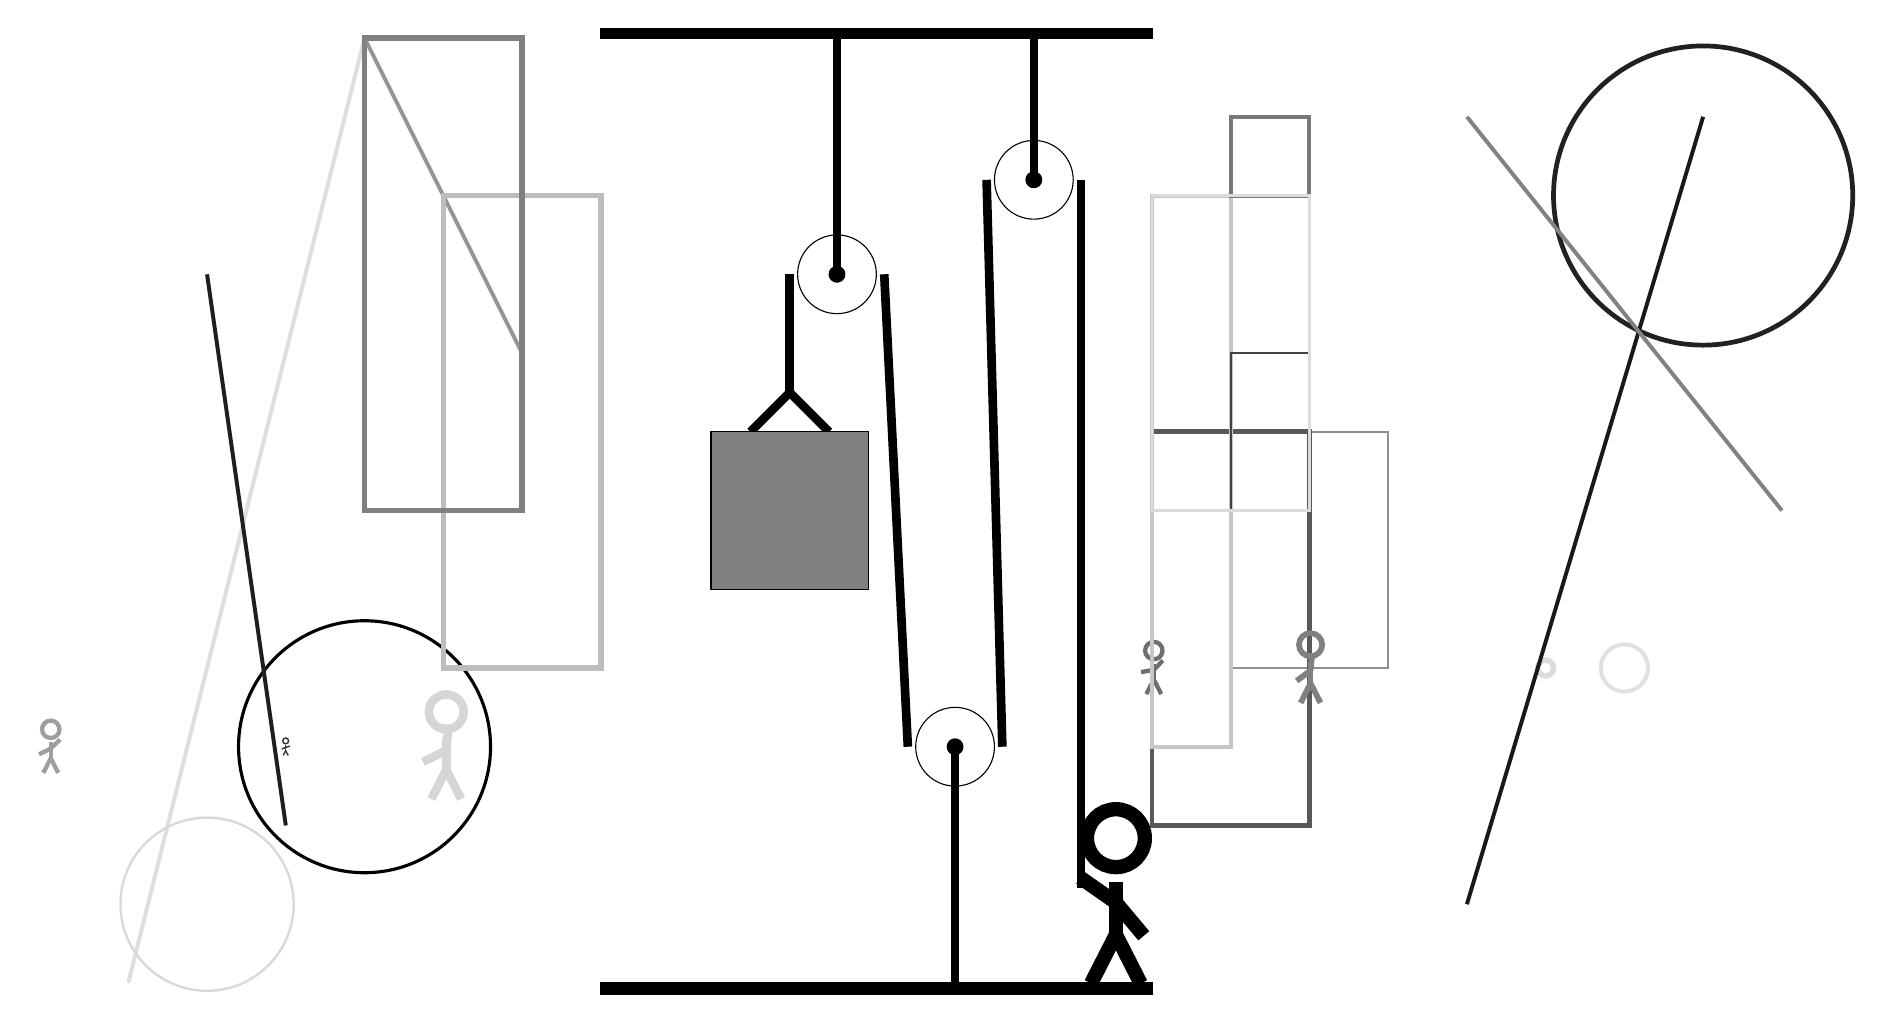
\begin{tikzpicture}
			%%%%% START %%%%%
			
			\draw[fill=black] (-2, 9) rectangle (5, 9.125);
			
			\draw (1, 6) circle (0.5);
			\draw[fill=black] (1, 6) circle (0.1);
			\draw[line width=1.1mm]  (1, 9) -- (1, 6);
			
			\draw[fill=white](2.5, 0) circle (0.5);
			\draw[fill=black] (2.5, 0) circle (0.1);
			\draw[line width=1.1mm]  (2.5, -3) -- (2.5, 0);
			
			\draw[fill=white](3.5, 7.2) circle (0.5);
			\draw[fill=black] (3.5, 7.2) circle (0.1);
			\draw[line width=1.1mm] (3.5, 9) -- (3.5, 7.2);
			
			\draw[line width=1.1mm] (-0.1, 4.0) -- (0.4, 4.5) -- (0.9, 4.0);
			\draw[fill=black!50] (-0.6, 4.0) rectangle (1.4, 2.0);
			
			\draw[line width=1.1mm] (0.4, 6) -- (0.4, 4.5);
			\centerarc[line width=1.1mm](1, 6)(0:180:0.6);
			\draw[line width=1.1mm](1.6, 6) -- (1.9, 0);
			\centerarc[line width=1.1mm](2.5, 0)(180:360:0.6);
			\draw[line width=1.1mm](3.1, 0) -- (2.9, 7.2);
			\centerarc[line width=1.1mm](3.5, 7.2)(0:180:0.6);
			\draw[line width=1.1mm](4.1, 7.2) -- (4.1, -1.8);
			
			\draw[line width=0.5mm, color=black!41](-3, 5) -- (-5, 9);
			
			\draw [line width=0.3mm, color=black!69](8, 3) circle (0.0);
			\draw [line width=0.6mm, color=black!87](12, 7) circle (1.9);
			\draw [line width=0.4mm, color=black!100](-5, 0) circle (1.6);
			
			\draw[line width=0.5mm, color=black!13](-5, 9) -- (-8, -3);
			\node[line width=0.4mm, color=black!80] at (-6, 0) {\Strichmaxerl[1][24][16]};
			\draw[line width=0.5mm, color=black!88](-6, -1) -- (-7, 6);
			
			\draw [line width=0.7mm, color=black!14](10, 1) circle (0.1);
			\node[line width=0.3mm, color=black!38] at (-9, 0) {\Strichmaxerl[3][26][44]};
			\node[line width=0.3mm, color=black!57] at (5, 1) {\Strichmaxerl[3][10][46]};
			
			\draw [line width=0.5mm, color=black!12](11, 1) circle (0.3);
			
			\draw[line width=0.7mm, color=black!26] (-2, 1) rectangle (-4, 7);
			\draw[line width=0.3mm, color=black!43] (6, 1) rectangle (8, 4);
			\draw [line width=0.6mm, color=black!96](6, -1) circle (0.0);
			\draw[line width=0.6mm, color=black!65] (5, -1) rectangle (7, 4);
			\node[line width=0.4mm, color=black!50] at (7, 1) {\Strichmaxerl[4][37][84]};
			\draw[line width=0.5mm, color=black!22] (6, 0) rectangle (5, 7);
			\draw[line width=0.3mm, color=black!74] (7, 3) rectangle (6, 5);
			\node[line width=0.4mm, color=black!16] at (-4, 0) {\Strichmaxerl[6][26][85]};
			\draw[line width=0.7mm, color=black!50] (-3, 3) rectangle (-5, 9);
			\draw[line width=0.5mm, color=black!53] (6, 8) rectangle (7, 7);
			
			\draw[line width=0.5mm, color=black!90](9, -2) -- (12, 8);
			
			\draw[line width=0.3mm, color=black!14] (7, 3) rectangle (5, 7);
			\draw [line width=0.3mm, color=black!15](-7, -2) circle (1.1);
			\draw[line width=0.5mm, color=black!49](9, 8) -- (13, 3);
			
			
			\node at (4.5, -1.9) {\Strichmaxerl[10][-35][-50]};
			
			\draw[fill=black] (-2, -3) rectangle (5, -3.15);
			
			%%%%% END %%%%%
		\end{tikzpicture}
	\end{figure}	
\end{document}